
% ---
% Capitulo da Metodologia
% ---

\chapter{Metodologia}\label{cap_metodologia}

Texto da Metodologia Parágrafo Parágrafo Parágrafo Parágrafo Parágrafo Parágrafo Parágrafo Parágrafo Parágrafo Parágrafo Parágrafo Parágrafo Parágrafo Parágrafo Parágrafo Parágrafo Parágrafo Parágrafo Parágrafo Parágrafo Parágrafo Parágrafo Parágrafo Parágrafo Parágrafo Parágrafo Parágrafo Parágrafo Parágrafo Parágrafo 

\section{Título da Seção 1}

Detalhamento da metodologia a ser utilizada: caracterização da pesquisa, população, amostra, instrumentos de medida. 


Este parágrafo apresenta como referenciar a figura no texto, requisito obrigatório da ABNT.  Primeira opção, utilizando \texttt{autoref}: Ver a \autoref{fig1}. Segunda opção, utilizando  \texttt{ref}: Ver a Figura \ref{fig1}.

\begin{figure}[h] 
\centering 
\caption{Exemplo de gráfico}\label{fig1} 
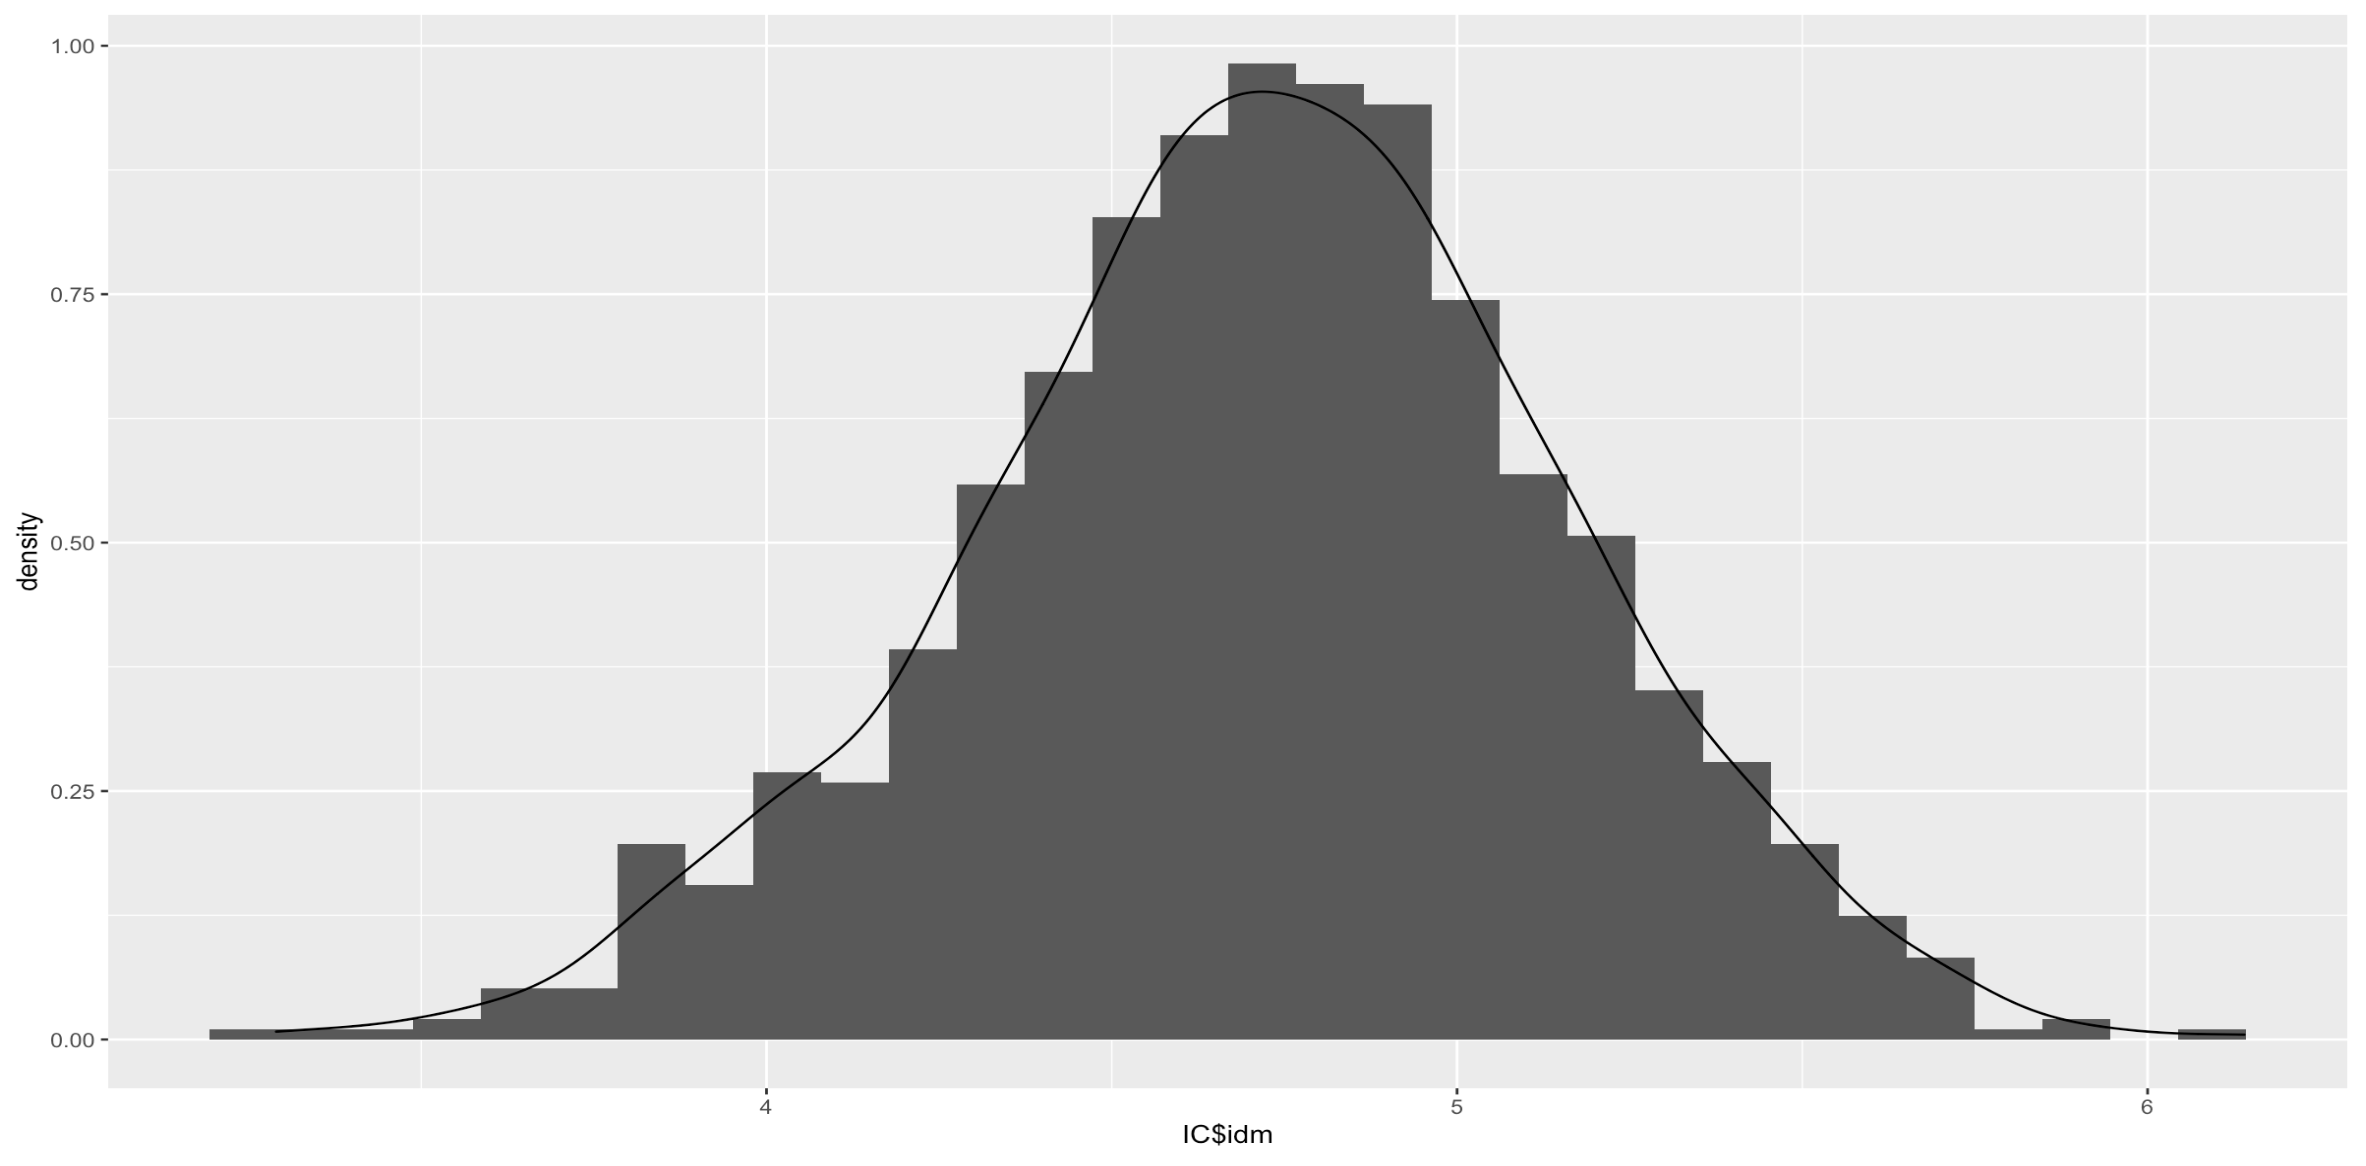
\includegraphics[scale=0.30]{figuras/hist.png}
\fonte{Elaborado pelo autor}
\end{figure}


Parágrafo Parágrafo Parágrafo Parágrafo Parágrafo Parágrafo Parágrafo Parágrafo Parágrafo Parágrafo Parágrafo Parágrafo Parágrafo Parágrafo Parágrafo Parágrafo Parágrafo Parágrafo Parágrafo Parágrafo Parágrafo Parágrafo Parágrafo Parágrafo Parágrafo Parágrafo Parágrafo Parágrafo Parágrafo Parágrafo 

Parágrafo Parágrafo Parágrafo Parágrafo Parágrafo Parágrafo Parágrafo Parágrafo Parágrafo Parágrafo Parágrafo Parágrafo Parágrafo Parágrafo Parágrafo Parágrafo Parágrafo Parágrafo Parágrafo Parágrafo Parágrafo Parágrafo Parágrafo Parágrafo 

Parágrafo Parágrafo Parágrafo Parágrafo Parágrafo Parágrafo Parágrafo Parágrafo Parágrafo Parágrafo Parágrafo Parágrafo Parágrafo Parágrafo Parágrafo Parágrafo Parágrafo Parágrafo Parágrafo Parágrafo Parágrafo Parágrafo Parágrafo Parágrafo Parágrafo Parágrafo Parágrafo Parágrafo 

\section{Título da Seção 2}

Parágrafo Parágrafo Parágrafo Parágrafo Parágrafo Parágrafo Parágrafo Parágrafo Parágrafo Parágrafo Parágrafo Parágrafo Parágrafo Parágrafo Parágrafo Parágrafo Parágrafo Parágrafo Parágrafo Parágrafo Parágrafo Parágrafo Parágrafo Parágrafo Parágrafo Parágrafo Parágrafo Parágrafo Parágrafo Parágrafo 

Parágrafo Parágrafo Parágrafo Parágrafo Parágrafo Parágrafo Parágrafo Parágrafo Parágrafo Parágrafo Parágrafo Parágrafo Parágrafo Parágrafo Parágrafo Parágrafo Parágrafo Parágrafo Parágrafo Parágrafo Parágrafo Parágrafo Parágrafo Parágrafo 

Parágrafo Parágrafo Parágrafo Parágrafo Parágrafo Parágrafo Parágrafo Parágrafo Parágrafo Parágrafo Parágrafo Parágrafo Parágrafo Parágrafo Parágrafo Parágrafo Parágrafo Parágrafo Parágrafo Parágrafo Parágrafo Parágrafo Parágrafo Parágrafo Parágrafo Parágrafo Parágrafo Parágrafo

\subsection{Título da Subseção}

Parágrafo Parágrafo Parágrafo Parágrafo Parágrafo Parágrafo Parágrafo Parágrafo Parágrafo Parágrafo Parágrafo Parágrafo Parágrafo Parágrafo Parágrafo Parágrafo Parágrafo Parágrafo Parágrafo Parágrafo Parágrafo Parágrafo Parágrafo Parágrafo Parágrafo Parágrafo Parágrafo Parágrafo Parágrafo Parágrafo 

Parágrafo Parágrafo Parágrafo Parágrafo Parágrafo Parágrafo Parágrafo Parágrafo Parágrafo Parágrafo Parágrafo Parágrafo Parágrafo Parágrafo Parágrafo Parágrafo Parágrafo Parágrafo Parágrafo Parágrafo Parágrafo Parágrafo Parágrafo Parágrafo 

Parágrafo Parágrafo Parágrafo Parágrafo Parágrafo Parágrafo Parágrafo Parágrafo Parágrafo Parágrafo Parágrafo Parágrafo Parágrafo Parágrafo Parágrafo Parágrafo Parágrafo Parágrafo Parágrafo Parágrafo Parágrafo Parágrafo Parágrafo Parágrafo Parágrafo Parágrafo Parágrafo Parágrafo
